% !TEX root = ../zavrsni_rad.tex

\chapter{Nelinearno modelsko prediktivno upravljanje}
\label{pog:nmpc}

\section{Što je MPC}

MPC (eng.\ \textit{Model Predictive Control}) \cite{rawlings2017mpc, borrelli2017predictive} na svakom koraku predviđa ponašanje sustava za sljedećih $N$ koraka i odabire upravljanje koje minimizira grešku u tom budućem prozoru, uz poštivanje svih ograničenja.

Analogno iskusnom vozaču koji gleda cestu 20 metara unaprijed: ne samo da uočava ono što dolazi, nego već sada planira buduće kočenje ili skretanje da problem riješi prije nego se pojavi.

Konkretno, na svakom koraku:
\begin{enumerate}
  \item izmjeri se trenutno stanje robota $(x, y, \theta, v, \omega)$
  \item optimizira se upravljanje za sljedećih $N = 20$ koraka ($= 2$ sekunde unaprijed)
  \item primijeni se samo \textbf{prvi} upravljački signal iz tog plana
  \item ponovi se u sljedećem koraku s novim mjerenjem
\end{enumerate}

Ovaj pristup se naziva klizni horizont (eng.\ \textit{receding horizon}): horizont se stalno pomiče naprijed zajedno s robotom. Prednost je što svako novo mjerenje automatski ispravlja akumulirane greške ili vanjske poremećaje.

\begin{figure}[H]
  \centering
  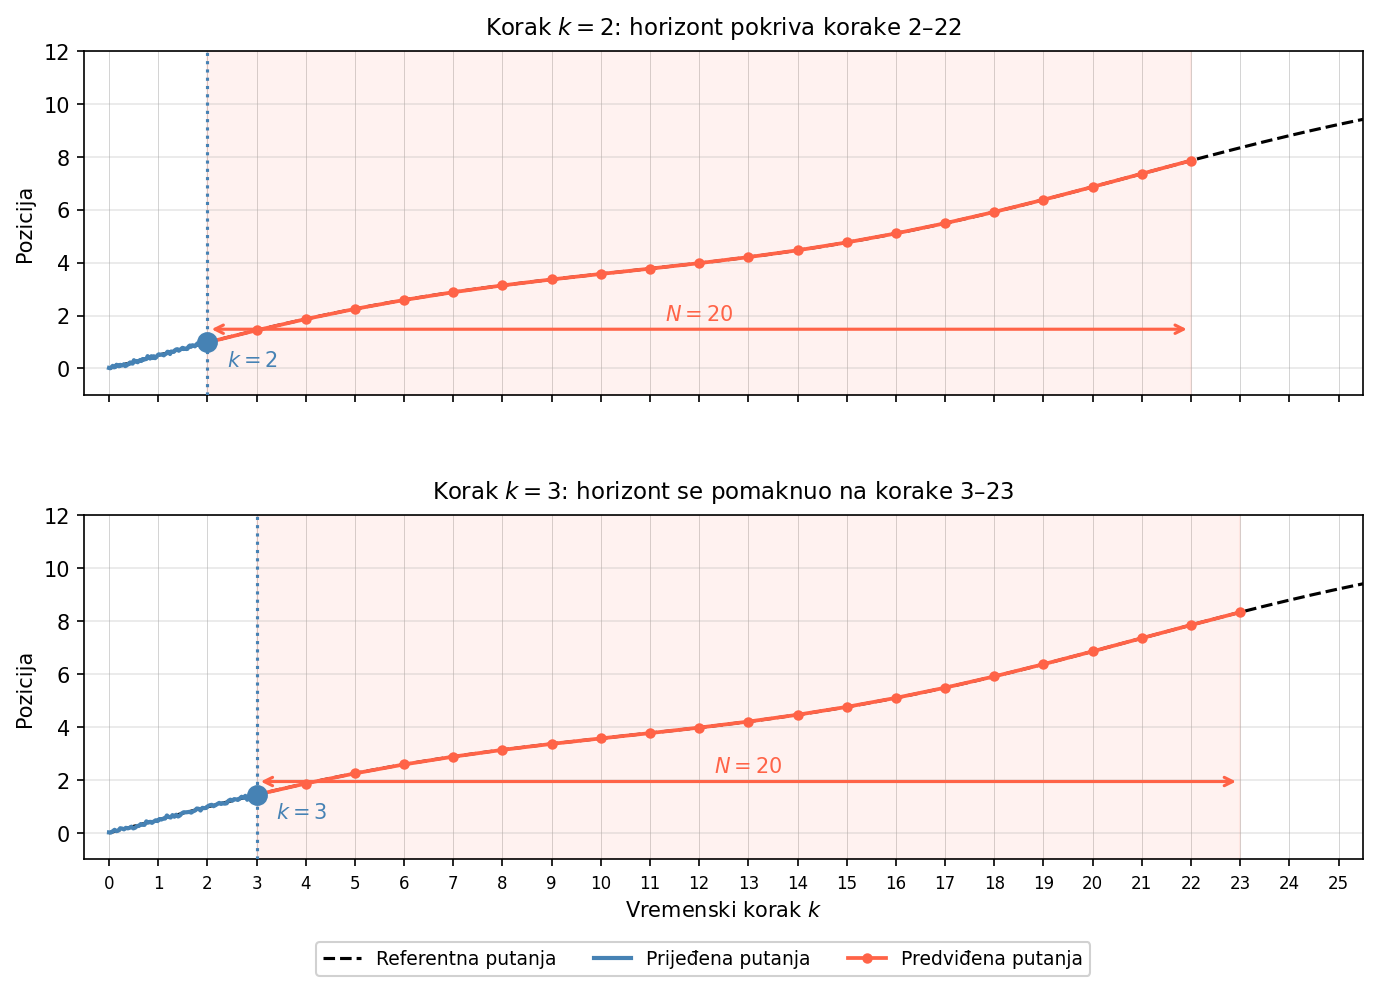
\includegraphics[width=0.95\linewidth]{figures/mpc_receding_horizon.png}
  \caption{Ilustracija kliznog horizonta. U koraku $k=2$ NMPC optimizira upravljanje za korake 2--22 (crveni segment, $N=20$). U sljedećem koraku $k=3$ horizont se pomiče naprijed na korake 3--23. Plava linija pokazuje prijeđenu putanju, a isprekidana crna referentnu.}
  \label{slk:receding_horizon}
\end{figure}

\textbf{Nelinearni MPC} (NMPC) je varijanta koja radi direktno s nelinearnim modelom. Jednokolica je nelinearna jer njezine jednadžbe kretanja sadrže $v\cos\theta$ i $v\sin\theta$ --- brzina i kut orijentacije su množeni, što sustav čini nelinearnim. Konkretno: robot koji vozi brzinom $v = 1$ m/s ravno ($\theta = 0$) kreće se isključivo u smjeru osi $x$, a isti robot koji vozi istom brzinom ali okrenut za $\theta = \pi/2$ kreće se isključivo u smjeru osi $y$ --- isti ulaz, potpuno drugačiji efekt ovisno o trenutnom stanju. Da je sustav linearan, način na koji upravljanje utječe na promjenu stanja bio bi konstantan i neovisan o trenutnoj orijentaciji. U monociklu naprotiv, faktori $\cos\theta$ i $\sin\theta$ množe brzinu $v$ --- isti upravljački signal pri različitom $\theta$ daje potpuno drugačiji smjer promjene pozicije. Zbog toga je potreban nelinearni optimizacijski pristup poput SQP-a.

\begin{figure}[H]
  \centering
  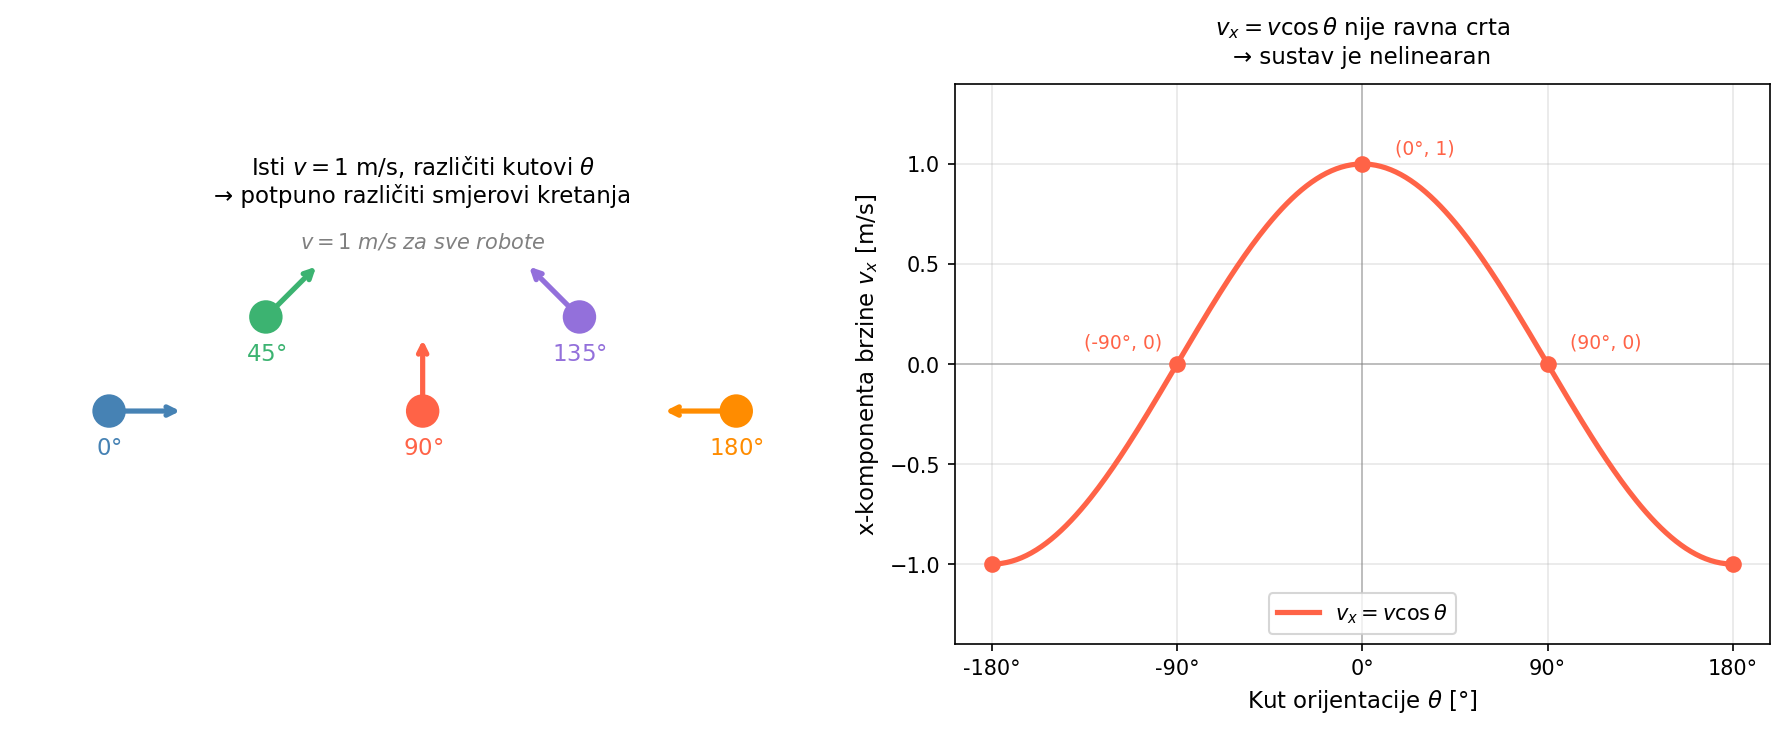
\includegraphics[width=0.95\linewidth]{figures/unicycle_nonlinear.png}
  \caption{Lijevo: robot pri istoj brzini $v=1$ m/s ali različitim kutovima orijentacije --- smjer kretanja potpuno se mijenja ovisno o stanju. Desno: x-komponenta brzine $v_x = v\cos\theta$ u ovisnosti o kutu --- valovita krivulja, ne ravna crta, što znači da je sustav nelinearan.}
  \label{slk:unicycle_nonlinear}
\end{figure}

\section{Formulacija optimizacijskog problema}

Cijeli NMPC problem može se zapisati kao optimizacijski problem s ograničenjima (OCP, eng.\ \textit{Optimal Control Problem}):

\begin{equation}
\label{eq:ocp}
\begin{aligned}
\min_{\substack{\mathbf{u}_0,\ldots,\mathbf{u}_{N-1} \\ \mathbf{s}_{0},\ldots,\mathbf{s}_{N-1}}} \quad
  & \sum_{k=0}^{N-1} \bigl\|\mathbf{y}_k - \mathbf{y}_{ref,k}\bigr\|^2_{W}
    + \bigl\|\mathbf{y}_N - \mathbf{y}_{ref,N}\bigr\|^2_{W_e}
    + \sum_{k=0}^{N-1} \sum_i \bigl( w_L\, s_{i,k} + w_Q\, s_{i,k}^2 \bigr) \\
\text{uz uvjet} \quad
  & \mathbf{x}_{k+1} = \Phi(\mathbf{x}_k, \mathbf{u}_k), \quad k = 0,\ldots,N-1 \\
  & \mathbf{x}_0 = \mathbf{x}_{meas} \\
  & |a_{v,k}| \leq 0{,}5 \ \text{m/s}^2, \quad |\alpha_k| \leq 1{,}0 \ \text{rad/s}^2 \\
  & 0{,}05 \leq v_k \leq 1{,}0 \ \text{m/s}, \quad |\omega_k| \leq 1{,}5 \ \text{rad/s} \\
  & h_i(\mathbf{x}_k) + s_{i,k} \geq 0, \quad s_{i,k} \geq 0
\end{aligned}
\end{equation}

gdje $\Phi(\mathbf{x}_k, \mathbf{u}_k)$ označava numerički integrator dinamike s korakom $\Delta t = 0{,}1$ s (konkretno ERK4 (eng.\ \textit{Explicit Runge-Kutta}, ERK) --- eksplicitna Runge-Kutta metoda 4.\ reda), $h_i(\mathbf{x}) = \|\mathbf{p} - \mathbf{c}_i\|_2 - r_i$ je udaljenost centra robota $\mathbf{p} = (x, y)$ od granice prepreke $i$ (centar $\mathbf{c}_i$, polumjer $r_i$), a $s_{i,k} \geq 0$ su slack varijable koje dopuštaju meka kršenja ograničenja prepreka uz kaznu $w_L = w_Q = 10^4$.

Sljedeće sekcije opisuju detaljno svaki od sastavnih dijelova ovog problema.

\section{Funkcija troška}

Na svakom koraku NMPC traži upravljačku sekvencu $\mathbf{u}_0, \ldots, \mathbf{u}_{N-1}$ koja minimizira kvadratnu funkciju troška:

\begin{equation}
  \min_{\mathbf{u}_0,\, \ldots,\, \mathbf{u}_{N-1}} \sum_{k=0}^{N-1} \|\mathbf{y}_k - \mathbf{y}_{ref,k}\|^2_W + \|\mathbf{y}_N - \mathbf{y}_{ref,N}\|^2_{W_e}
\end{equation}

gdje je $\mathbf{y}_k$ izlazni vektor koji kombinira stanja i upravljanje, a $\mathbf{y}_{ref,k}$ referentni vektor koji dolazi s A* putanje:

\begin{equation}
  \mathbf{y}_k = \begin{bmatrix} x_k \\ y_k \\ \theta_k \\ a_{v,k} \\ \alpha_k \end{bmatrix}, \qquad
  \mathbf{y}_{ref,k} = \begin{bmatrix} x_{ref} \\ y_{ref} \\ \theta_{ref} \\ 0 \\ 0 \end{bmatrix}
\end{equation}

Nule na kraju $\mathbf{y}_{ref,k}$ znače da su željena ubrzanja nula --- robot treba mijenjati brzinu samo koliko je nužno za praćenje putanje. Matrica troška $W$ blok-dijagonalne je strukture:

\begin{equation}
  W = \begin{bmatrix} Q & 0 \\ 0 & R \end{bmatrix}, \qquad
  Q = \begin{bmatrix} 10{,}0 & 0 & 0 \\ 0 & 10{,}0 & 0 \\ 0 & 0 & 1{,}0 \end{bmatrix}, \qquad
  R = \begin{bmatrix} 0{,}1 & 0 \\ 0 & 0{,}1 \end{bmatrix}
\end{equation}

Omjer dijagonalnih elemenata $Q_{xx} / R_{a_v} = 10{,}0 / 0{,}1 = 100$ znači da je korekcija pozicije 100 puta važnija od glatkoće upravljanja. Terminalna matrica $W_e = Q$ kažnjava grešku na kraju horizonta istim težinama --- odabir $W_e = Q$ je heuristički i u praksi se pokazao stabilnim, no postoje i sofisticiranije metode (npr.\ rješavanje Riccatijeve jednadžbe).

Ove vrijednosti nisu odabrane nasumično --- u poglavlju~\ref{pog:rezultati} prikazana je analiza kako različiti omjeri $Q/R$ utječu na preciznost praćenja.

Izlazni vektor $\mathbf{y}_k$ dobiva se linearnom projekcijom stanja i upravljanja: $\mathbf{y}_k = V_x \mathbf{x}_k + V_u \mathbf{u}_k$, gdje su projekcijske matrice:

\begin{equation}
  V_x = \begin{bmatrix}
    1 & 0 & 0 & 0 & 0 \\
    0 & 1 & 0 & 0 & 0 \\
    0 & 0 & 1 & 0 & 0 \\
    0 & 0 & 0 & 0 & 0 \\
    0 & 0 & 0 & 0 & 0
  \end{bmatrix}, \qquad
  V_u = \begin{bmatrix}
    0 & 0 \\
    0 & 0 \\
    0 & 0 \\
    1 & 0 \\
    0 & 1
  \end{bmatrix}
\end{equation}

Gornje tri komponente izlaza ($x$, $y$, $\theta$) dolaze iz vektora stanja, a donje dvije ($a_v$, $\alpha$) iz vektora upravljanja. Odgovarajuća implementacija u acadosu:

\begin{listing}[H]
\begin{minted}{python}
Q = np.diag(mpc["Q"])   # diag(10, 10, 1) -- x, y, theta
R = np.diag(mpc["R"])   # diag(0.1, 0.1)  -- dv, domega

ocp.cost.Vx = np.zeros((ny, nx))
ocp.cost.Vx[:3, :3] = np.eye(3)    # uzmi x, y, theta iz stanja

ocp.cost.Vu = np.zeros((ny, nu))
ocp.cost.Vu[3:, :] = np.eye(nu)    # uzmi dv, domega iz upravljanja

ocp.cost.W   = np.block([[Q, np.zeros((3, nu))],
                          [np.zeros((nu, 3)), R]])
ocp.cost.W_e = Q                    # terminalna matrica = Q
\end{minted}
\caption{Postavljanje matrica troška u \texttt{src/mpc\_solver.py}}
\end{listing}

\section{Ograničenja}

Sva fizikalna ograničenja robota direktno su ugrađena u optimizacijski problem. Ograničenja na upravljanje (maksimalna ubrzanja):

\begin{equation}
  |a_v| \leq 0{,}5 \ \text{m/s}^2, \qquad |\alpha| \leq 1{,}0 \ \text{rad/s}^2
\end{equation}

Ograničenja na stanja (fizikalne granice robota i okolina):

\begin{equation}
  0{,}05 \leq v \leq 1{,}0 \ \text{m/s}, \qquad |\omega| \leq 1{,}5 \ \text{rad/s}
\end{equation}
\begin{equation}
  0 \leq x \leq 10 \ \text{m}, \qquad 0 \leq y \leq 10 \ \text{m}
\end{equation}

Implementacija u \texttt{src/mpc\_solver.py}:

\begin{listing}[H]
\begin{minted}{python}
ocp.constraints.lbu = np.array([-robot["dv_max"], -robot["domega_max"]])  # dv, domega min
ocp.constraints.ubu = np.array([ robot["dv_max"],  robot["domega_max"]])  # dv, domega max

ocp.constraints.lbx = np.array([env["x_min"], env["y_min"], -np.pi,
                                 robot["v_min"], -robot["omega_max"]])     # donje granice stanja
ocp.constraints.ubx = np.array([env["x_max"], env["y_max"],  np.pi,
                                 robot["v_max"],  robot["omega_max"]])     # gornje granice stanja
\end{minted}
\caption{Postavljanje ograničenja u \texttt{src/mpc\_solver.py}}
\end{listing}

\section{Meka ograničenja izbjegavanja prepreka}

Za svaku kružnu prepreku s centrom $(c_x, c_y)$ i polumjerom $r$ definira se uvjet sigurnosne udaljenosti:

\begin{equation}
  h(\mathbf{x}) = (x - c_x)^2 + (y - c_y)^2 - (r + r_{rob})^2 \geq 0
\end{equation}

gdje je $r_{rob} = 0{,}2$ m polumjer robota. Ovaj uvjet mora biti zadovoljen za svaki korak horizonta.

Ograničenja su implementirana kao \textbf{meka} (eng.\ \textit{soft}): umjesto da se zahtijeva $h_i(\mathbf{x}_k) \geq 0$, uvodi se slack varijabla $s_{i,k} \geq 0$ i relaksirani uvjet postaje:

\begin{equation}
  h_i(\mathbf{x}_k) + s_{i,k} \geq 0, \qquad s_{i,k} \geq 0
\end{equation}

Kada je $s_{i,k} = 0$, ograničenje je zadovoljeno; kada je $s_{i,k} > 0$, robot je unutar sigurnosne zone prepreke $i$ i veličina $s_{i,k}$ mjeri iznos kršenja. Svaka slack varijabla kažnjava se u funkciji troška linearnim i kvadratnim penalom:

\begin{equation}
  \sum_{k=0}^{N-1} \sum_i \bigl( w_L\, s_{i,k} + w_Q\, s_{i,k}^2 \bigr), \qquad w_L = w_Q = 10^4
\end{equation}

Linearna komponenta pokreće robot iz prepreke čak i kod malih kršenja, a kvadratna brzo raste s većim kršenjima. Meka formulacija korisna je jer održava numeričku rješivost OCP-a u uskim prostorima i pri nesavršenim referencama --- tvrda ograničenja bi u takvim situacijama uzrokovala neriješivost solvera.

\begin{listing}[H]
\begin{minted}{python}
for (cx, cy, r) in obstacles:
    # h(x) = (x-cx)^2 + (y-cy)^2 - (r + r_robot)^2 >= 0
    h_list.append((px - cx)**2 + (py - cy)**2 - (r + r_robot)**2)

ocp.model.con_h_expr = ca.vertcat(*h_list)   # nelinearna ograničenja za acados

penalty = 1e4                                  # kazna za kršenje ograničenja
ocp.cost.zl = penalty * np.ones(n_obs)        # linearni penalty
ocp.cost.Zl = penalty * np.ones(n_obs)        # kvadratni penalty
\end{minted}
\caption{Implementacija mekih ograničenja prepreka u \texttt{src/mpc\_solver.py}}
\end{listing}

\section{SQP\_RTI solver}

Za rješavanje nelinearnog optimizacijskog problema na svakom koraku koristi se SQP\_RTI (eng.\ \textit{Sequential Quadratic Programming --- Real-Time Iteration}) pristup unutar alata acados \cite{verschueren2022acados, acados_docs, diehl2002rti}.

SQP (eng.\ \textit{Sequential Quadratic Programming}) je metoda optimizacije koja iterativno linearizira nelinearni problem i rješava niz kvadratičnih potprograma. SQP\_RTI (eng.\ \textit{Real-Time Iteration}) je varijanta prilagođena za primjene u stvarnom vremenu i sastoji se od dvije faze koje se izmjenjuju u svakom regulacijskom koraku \cite{diehl2002rti}:

\begin{enumerate}
  \item \textbf{Faza pripreme} (eng.\ \textit{preparation phase}): linearizacija dinamike duž trenutne trajektorije, izračun Jacobijana, kondenzacija kvadratičnog potprograma (eng.\ \textit{Quadratic Program}, QP) --- ove operacije odvijaju se \textit{unaprijed}, dok robot još izvršava prethodni upravljački signal.
  \item \textbf{Faza povratne veze} (eng.\ \textit{feedback phase}): čim stigne novo mjerenje $\mathbf{x}_{meas}$, postavi se inicijalni uvjet i izvrši jedna SQP iteracija rješavanjem pripremljenog QP-a. Rezultat je novi upravljački signal koji se odmah šalje robotu.
\end{enumerate}

Zahvaljujući ovoj podjeli, kašnjenje između mjerenja i primjene upravljanja iznosi samo trajanje feedback faze (najmanji dio ukupnog računanja), dok se skuplja priprema odvija paralelno s izvođenjem prethodnog koraka.

Za rješavanje kvadratičnog potprograma unutar svake SQP iteracije koristi se HPIPM rješavač (eng.\ \textit{High Performance Interior Point Method}) koji je optimiziran za strukturu MPC problema. Gauss-Newtonova aproksimacija hesijana zamjenjuje pravi hesijan Lagrangiana aproksimacijom $J^\top W J$, gdje je $J$ Jacobijan reziduala (razlika $\mathbf{y}_k - \mathbf{y}_{ref,k}$) kvadratne funkcije troška, a $W$ težinska matrica. Time se izbjegava skupo računanje drugih derivacija nelinearne dinamike i ograničenja uz cijenu blago slabije konvergencije --- za RTI shemu s jednom iteracijom po koraku to je prihvatljiv kompromis.

Ukupno vrijeme rješavanja po koraku izmjereno u eksperimentima iznosi između $0{,}09$ i $0{,}12$ ms --- daleko ispod vremenskog koraka od $100$ ms, što ostavlja dovoljno prostora za opterećenje komunikacije i perifernih operacija.

\begin{listing}[H]
\begin{minted}{python}
ocp.solver_options.nlp_solver_type = mpc["solver_type"]   # "SQP_RTI"
ocp.solver_options.qp_solver       = "PARTIAL_CONDENSING_HPIPM"
ocp.solver_options.hessian_approx  = "GAUSS_NEWTON"
ocp.solver_options.integrator_type = "ERK"                # eksplicitni Runge-Kutta 4. reda
ocp.solver_options.nlp_solver_max_iter = 50
\end{minted}
\caption{Konfiguracija SQP\_RTI solvera u \texttt{src/mpc\_solver.py}}
\end{listing}
